\thispagestyle{empty}
\chapter{Paléovirologie et étude des éléments viraux endogénisés}
{\hypersetup{linkcolor=GREYDARK}\minitoc}
\label{chap:intro-EVES_dEVEs}
\newpage

\section{Le monde singulier des virus}

\subsection{La biologie des virus}

À ma connaissance, toutes les formes de vie cellulaire ont des génomes à ADN double brins (dsDNA) et suivent les mêmes règles de réplication et d'expression. Les virus, quant à eux, utilisent toutes les structures génomiques possibles (\figurename{\ref{figure:Structures_genomiques_virale}}). En effet, les virus ont des génomes constitués d'ADN ou d'ARN, circulaires ou linéaires, et constitués d'une ou plusieurs molécules. 

\begin{figure}[!htpb]
\captionsetup{font=footnotesize}
 \centering
  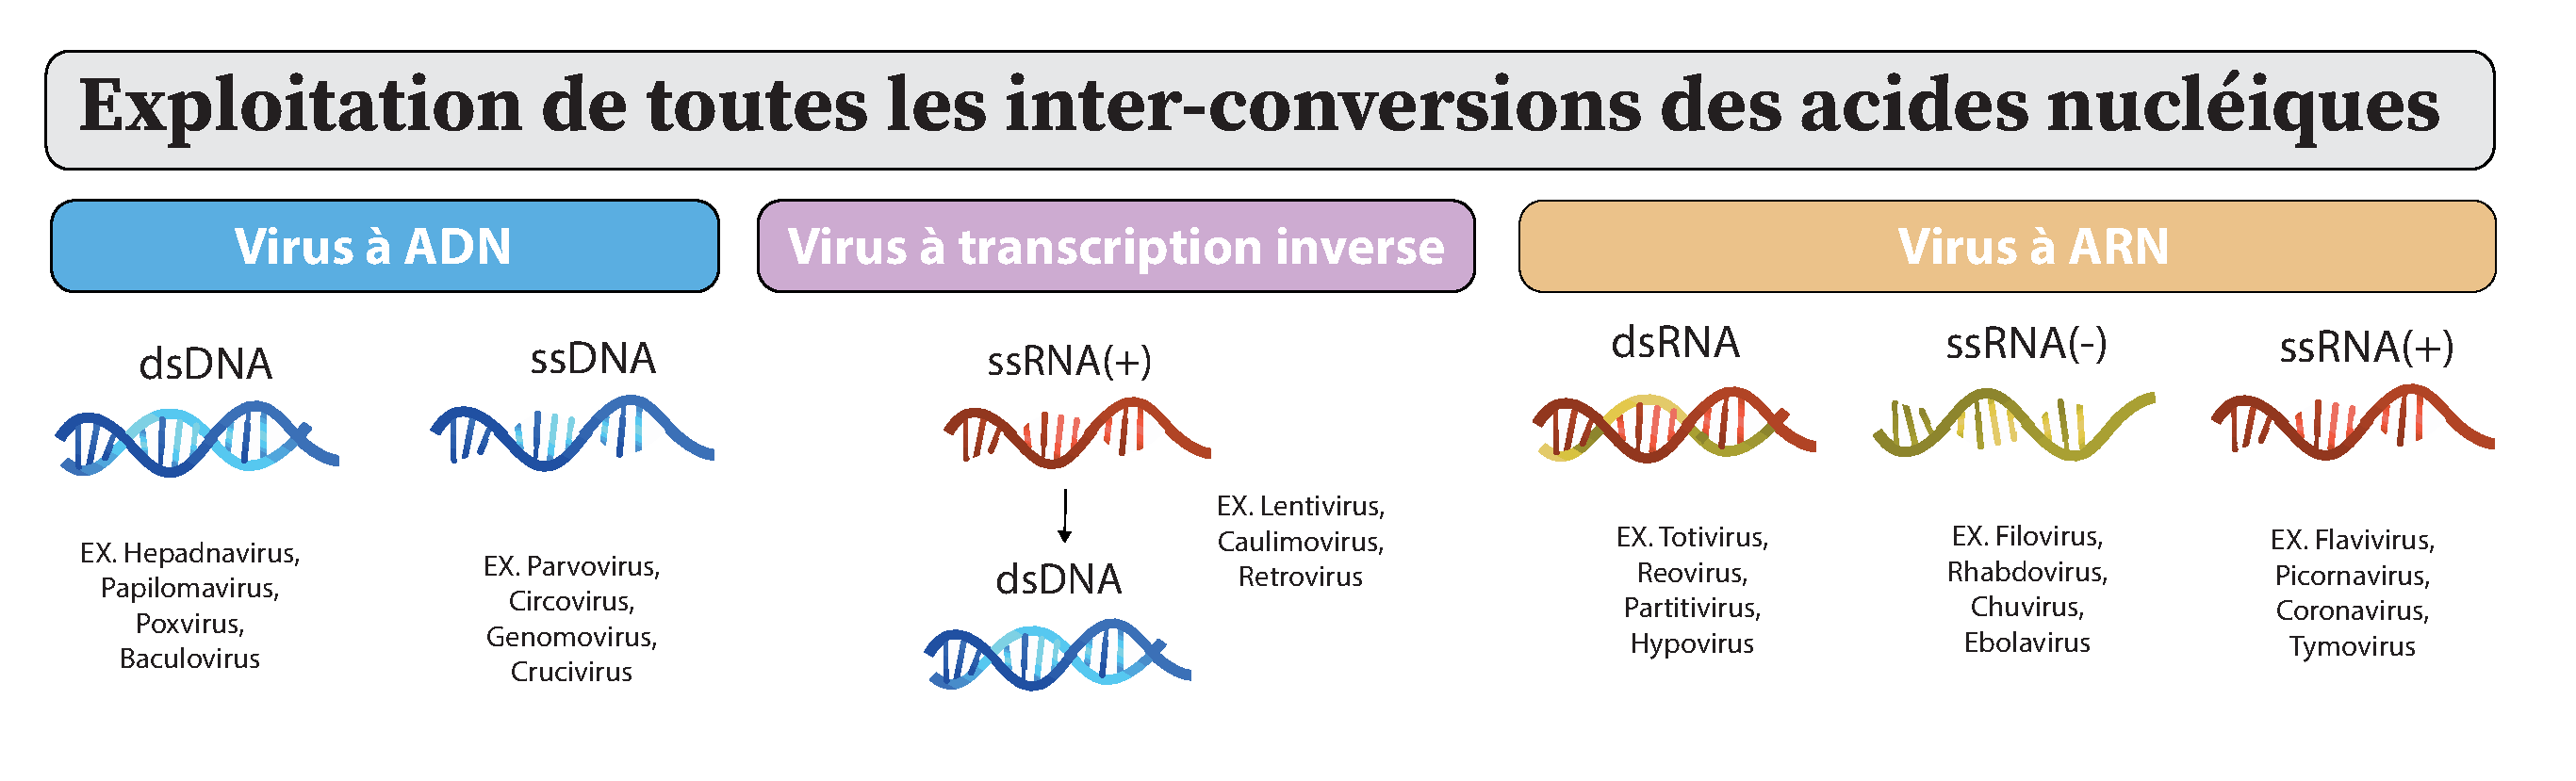
\includegraphics[width=\linewidth,height=\textheight,keepaspectratio]{PhD-master/figures/Structures_genomiques_virales.pdf}
\caption[Intro:Schéma récapitulatif de toutes les structures génomiques virales]{\textbf{Schéma récapitulatif de toutes les structures génomiques virales} }
\label{figure:Structures_genomiques_virale}
\end{figure}

Tous les virus sont des parasites intracellulaires obligatoires, ce qui signifie qu'ils produisent de nouvelles particules virales infectieuses, ou virions, à l'intérieur de la cellule. Bien entendu, les virus ont de nombreuses stratégies d'infection et des biologies différentes, mais il existe quelques généralités. Pour pénétrer dans une cellule, tous les virus doivent par exemple se lier à sa surface. Le virus se décapside alors et son matériel génétique, qui code pour des protéines, va spontanément former de nouveaux virions, après un cycle de réplication \textit{de novo}. Contrairement aux cellules, qui se divisent en deux pour se répliquer, les virus utilisent l'énergie et la machinerie de la cellule pour créer et assembler de nouveaux virions.

Pour infecter d'autres cellules, la particule virale mature doit s'échapper de la cellule hôte. Qu'il s'agisse de virus dsDNA, ssDNA, dsRNA ou ssRNA, le génome du virus évolue dans un environnement hostile. La capside (\figurename{\ref{figure:Structure_virale}}) protège donc l'acide nucléique de tous les virus. Chez certains virus, une enveloppe lipidique protège également la capside (\figurename{\ref{figure:Structure_virale}}). La couche la plus externe de chaque virus contient des protéines d'attachement qui lui permettent, grâce à leur capacité fusogénique, de se fixer à la membrane plasmique de la cellule hôte et de finalement fusionner leurs membranes. Cette fusion membranaire permet au virus de pénétrer dans la cellule. 


\begin{figure}[!htpb]
\captionsetup{font=footnotesize}
 \centering
  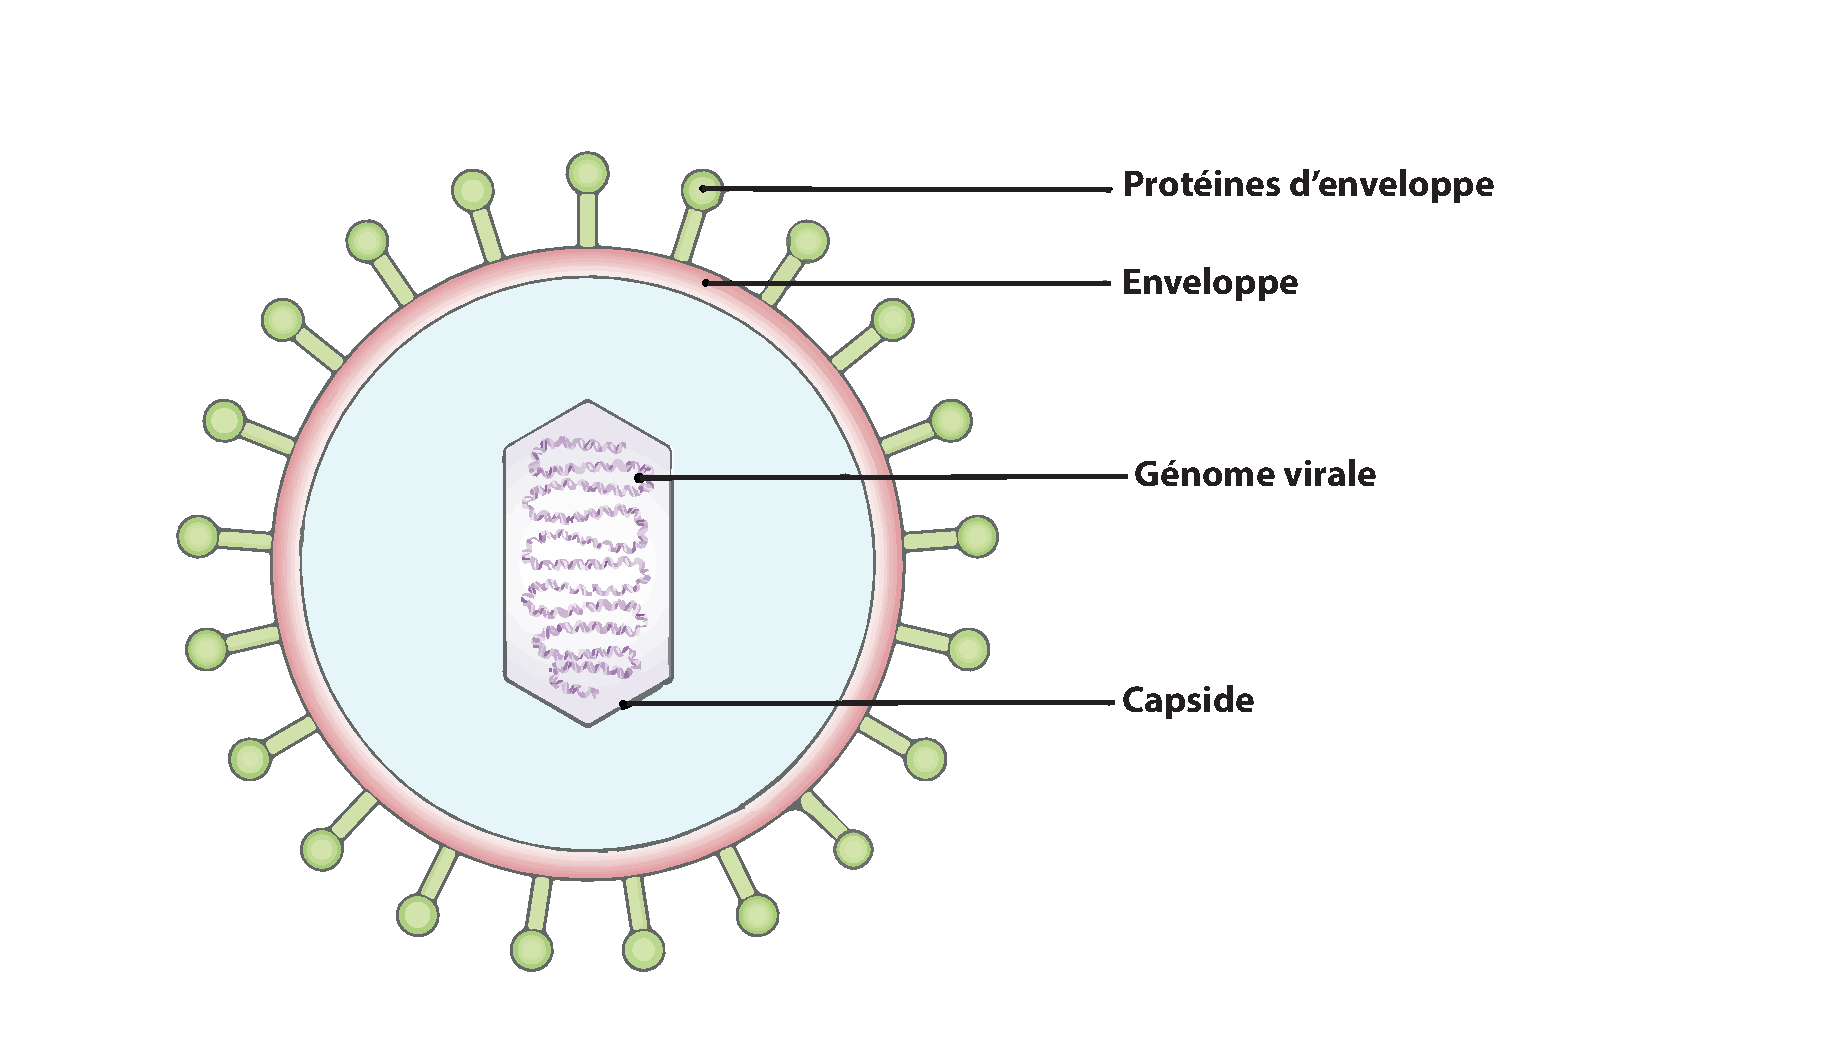
\includegraphics[width=\linewidth,height=\textheight,keepaspectratio]{PhD-master/figures/Structure_virale.pdf}
\caption[Intro:Structure virale générale]{\textbf{Structure virale générale}.}
\label{figure:Structure_virale}
\end{figure}

Contrairement aux génomes cellulaires, les génomes viraux sont très petits (\figurename{\ref{figure:Taille_et_mutations_virales}}). Ainsi, les virus à ARN possèdent les génomes les plus petits (la longueur moyenne du génome de virus ARN le plus petit n'est que de 9kb). Ces petits génomes présentent souvent des taux de mutation plus élevés (\figurename{\ref{figure:Taille_et_mutations_virales}}) \citep{gago_extremely_2009}.

\begin{figure}[!htpb]
\captionsetup{font=footnotesize}
 \centering
  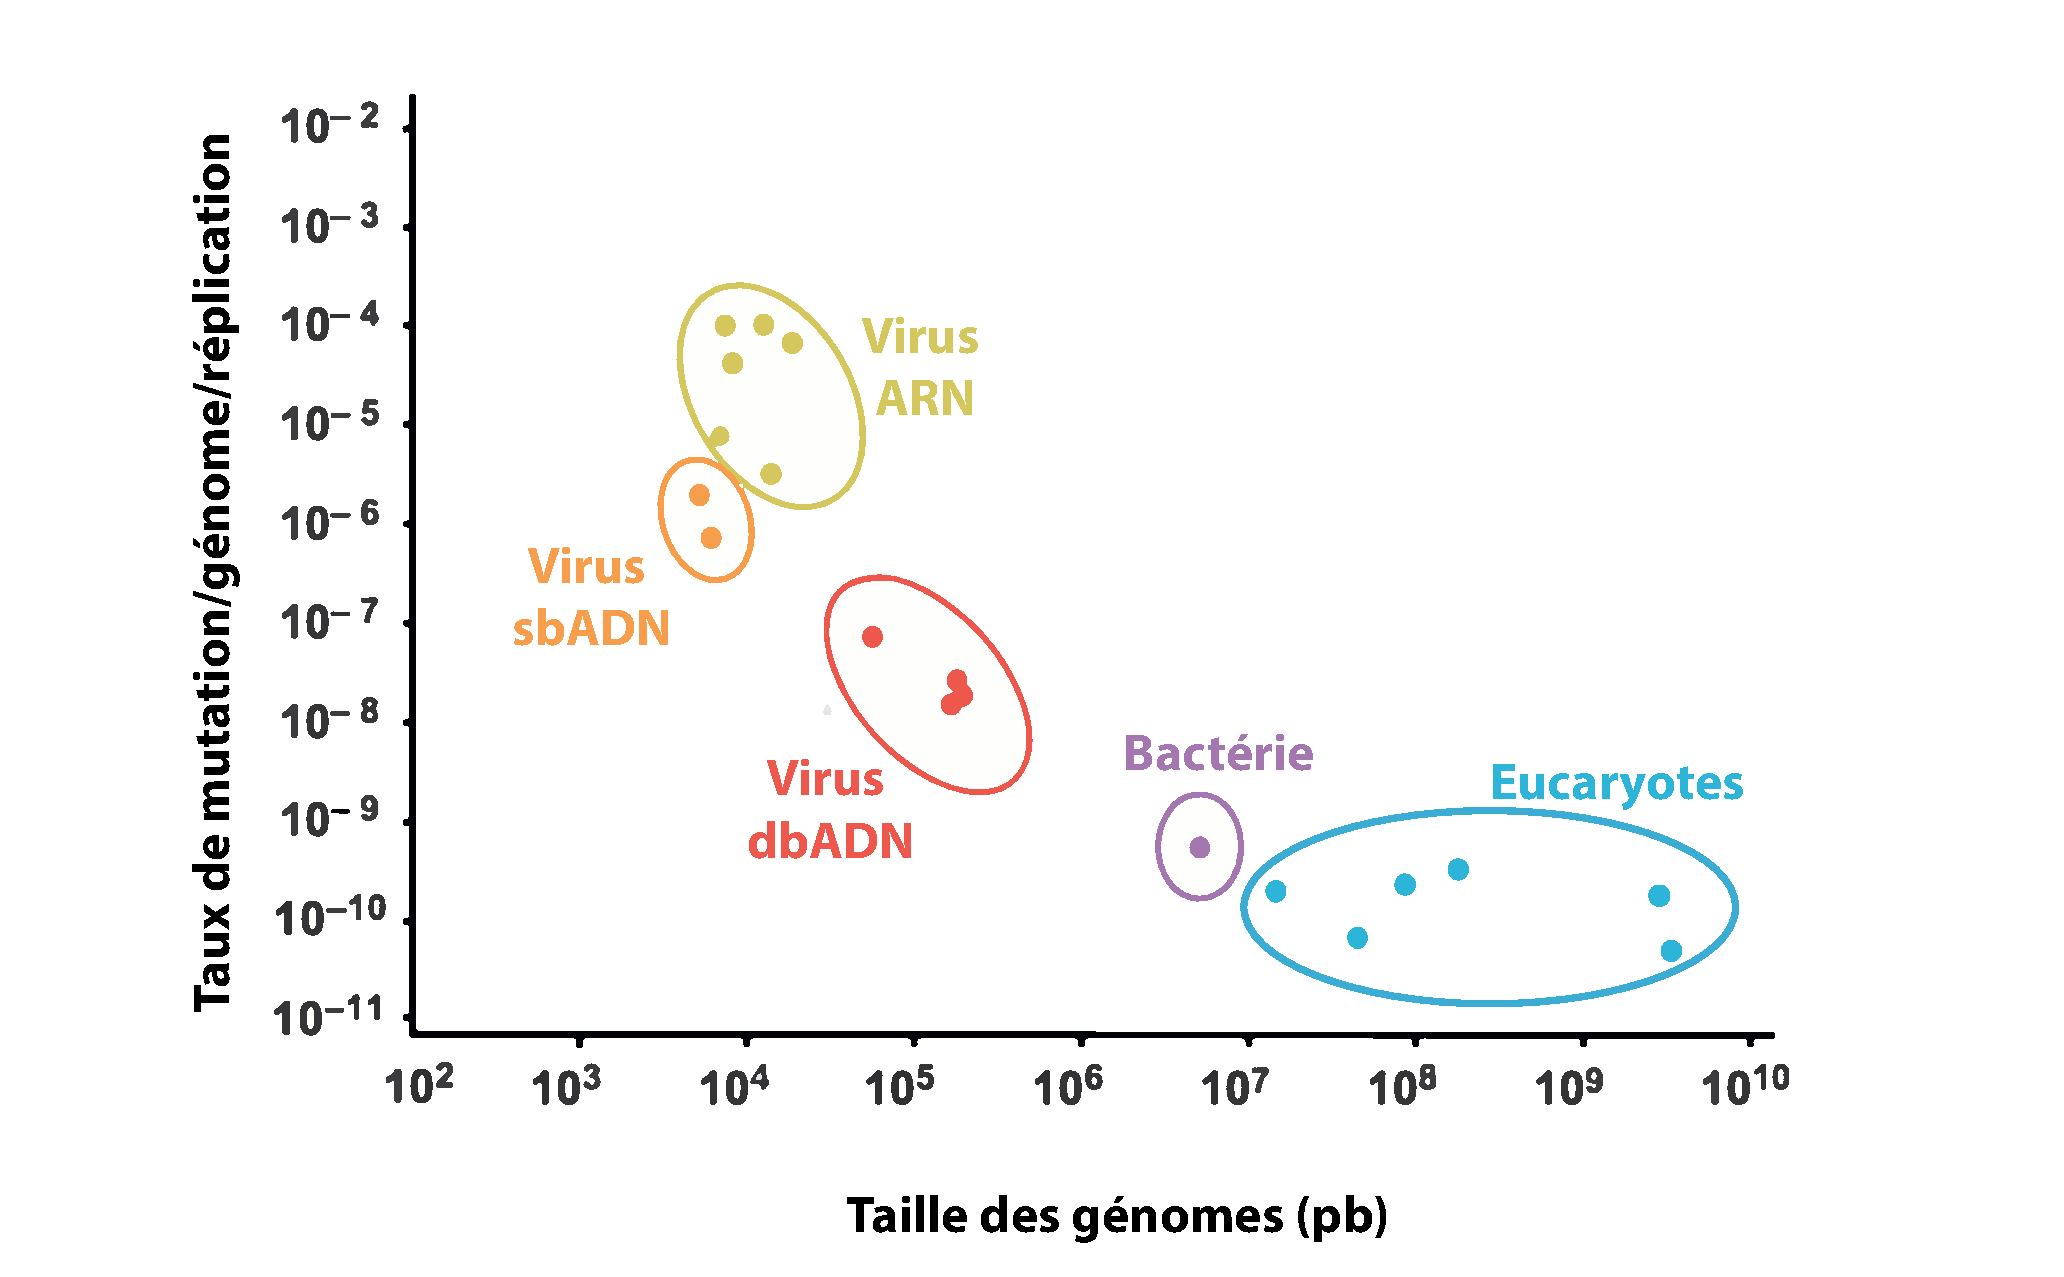
\includegraphics[width=\linewidth,height=\textheight,keepaspectratio]{PhD-master/figures/Taille_et_mutations_virales.pdf}
\caption[Intro:Distribution des taux de mutation en fonction de la taille du génome]{\textbf{Taux de mutation par site en fonction de la taille du génome pour différentes entités biologiques modifié de \cite{gago_extremely_2009}}.}
\label{figure:Taille_et_mutations_virales}
\end{figure}


\subsection{La symbiose}


Les associations symbiotiques entre les symbiotes et leurs hôtes fluctuent selon un continuum allant du parasitisme jusqu’au mutualisme. À ce titre, les virus sont par définition des symbiotes dans la mesure où ils se reproduisent aux dépens d'une cellule hôte. En conséquence, l'évolution de la virulence des virus peut être abordée à la lumière des modèles généraux qui ont été développés sur d'autres modèles symbiotiques, en particulier bactériens. Dans ce modèle, on définit la virulence comment étant la réduction de fitness induite par le symbiote sur son hôte. L'évolution de la virulence est alors principalement gouvernée par le mode de transmission des symbiotes \citep{smith_geneseye_2007}. En cas de transmission horizontale, la sélection est susceptible de favoriser des symbiotes virulents du fait de ce découplage entre les fitness des symbiotes et  de leurs hôtes. À l'inverse, une transmission verticale des symbiotes des parents hôtes à leur progéniture sélectionnera plutôt des symbiotes de moindre virulence, voir ayant un effet bénéfique sur la fitness de leurs hôtes. Dans ce dernier cas, on parle de mutualisme.

Les virus ont tous en général une composante horizontale pour leur transmission, ce qui va favoriser l'évolution de la virulence. Cette virulence peut être forte comme dans le cas du virus Ebola qui se transmet très efficacement entre individus et induit un taux de mortalité très élevé à son hôte \citep{kadanali_overview_2016}. 

En dehors de ces virus à transfert horizontal, d'autres virus présentent à la fois des modes de transmission horizontaux et également verticaux. Dans ce cas-là, la fitness du virus est donc en grande partie liée à son hôte, ce qui sélectionne pour une moindre virulence. Un tel exemple peut être retrouvé chez le virus LbFV (pour Leptopilina boulardi filamentous virus)  qui infecte la guêpe parasitoïde \textit{Leptopilina boulardi}. Ces virus sont transmis principalement verticalement de la mère aux progénitures. Cependant, des transferts horizontaux sont également observés. En effet, LbFV manipule le comportement de ponte des guêpes \textit{Leptopilina boulardi} en induisant du superparasitisme (ponte des œufs chez des hôtes déjà parasités) \citep{varaldi_infectious_2003,varaldi_artifical_2006}. Cette modification comportementale favorise ainsi la transmission horizontale du virus au sein des hôtes diptères superparasités, permettant une propagation efficace du virus dans les populations de guêpes \citep{gandon_superparasitism_2006}. 

Enfin, certains virus présentent plutôt une relation mutualiste avec leurs hôtes, comme le cas d'un entomopoxvirus se répliquant dans la guêpe parasitoïde \textit{Diachasmimorpha longicaudata} (DlEPV). Ce virus mutualiste est transmis verticalement et donne aux guêpes \textit{D. longicaudata} un avantage en termes de fitness en favorisant le succès reproducteur lors d'une infestation chez un hôte diptère \citep{coffman_genomic_2020}. Enfin, il existe également une forme de mutualisme plus poussée - on pourrait même parler d'un paroxysme symbiotique - qui implique les virus sous une forme intégrée dans les génomes de leurs hôtes (éléments viraux endogènes ou EVEs), comme dans le cas du gène d'enveloppe \textit{env} de rétrovirus, endogène chez les mammifères, qui permet la formation du syncitium \citep{lavialle_paleovirology_2013}.

\section{Les Éléments viraux endogènes (EVEs)}

\subsection{Historique}

Outre leurs propriétés infectieuses qui permettent aux virus de se propager de manière horizontale entre individus et entre espèces, il peut arriver qu'un virus s'intègre au matériel génétique de l'hôte via un processus connu sous le nom d'endogénisation \citep{katzourakis_endogenous_2010}. Ce phénomène d'endogénisation génère l'apparition de ce qu'on appelle des "Endogenous Viral Elements", en français "Eléments Viraux Endogènes" (EVEs). Les intégrations virales dans les chromosomes de leurs hôtes  peuvent alors concerner de petits fragments de génomes viraux, jusqu'à des génomes viraux entiers \citep{feschotte_endogenous_2012}.\\

Les premières recherches sur les EVEs ont principalement porté sur les rétrovirus endogènes (\textit{Retroviridae}), abondants dans les génomes des vertébrés et des plantes \citep{johnson_origins_2019}. Si la majeure partie des EVEs retrouvés dans la littérature correspond à des intégrations virales provenant de rétrovirus, c'est notamment parce qu'il s'agit des seuls virus à nécessiter une intégration chromosomique pour réaliser leur cycle de vie complet. Cette propriété dérive du fait que leur génome code pour l'ensemble de la machinerie enzymatique nécessaire à l'intégration. Ainsi, lorsque les particules composées de copies d'ARN du génome viral pénètrent dans une cellule cible, elles sont retro-transcrites en une molécule d'ADN double brin et intégrées à l'ADN génomique de la cellule hôte. Le provirus qui en résulte (forme intégrée, aussi appelée ERV pour endogenous retrovirus) code toutes les protéines structurelles et les enzymes nécessaires à l'assemblage des virions de la progéniture, ainsi que les éléments régulateurs nécessaires à la transcription de l'ARN viral. Les rétrovirus infectent généralement les tissus somatiques et ne sont donc pas transmis aux générations suivantes.  Toutefois, l'intégration peut parfois se produire dans les cellules germinales, permettant la propagation dans une population hôte. Une fois transmises à la génération suivante, ces nouvelles insertions peuvent éventuellement se fixer dans la population, soit par dérive, soit par sélection \citep{johnson_origins_2019}.   

À la fin des années 1990 et au début des années 2000, des EVEs dérivant de virus non retroviraux ont été décrites dans diverses lignées d'eucaryotes \citep{katzourakis_endogenous_2010,belyi_sequences_2010,liu_widespread_2010}. Aussi, l’explosion des programmes de séquençage de génome a permis de révéler la fréquence et la diversité virale impliquée dans ces phénomènes d’endogénisation. Toutes sortes de virus ont pu être endogénisés chez toutes sortes d'organismes, que l’intégration dans les chromosomes de leur hôte fasse partie ou non de leur cycle de vie naturel \citep{feschotte_endogenous_2012,aiewsakun_endogenous_2015}. Chez les insectes par exemple, pour lesquels aucun rétrovirus n'a été décrit jusqu'à aujourd'hui, de nombreux travaux montrent que les génomes abondent d'EVEs non rétroviraux \citep{gilbert_diversity_2022,cheng_nudivirus_2020,flynn_assessing_2019}.\\

Les EVEs non rétroviraux peuvent dériver de virus ayant des génomes dsDNA \citep{di_giovanni_behavior-manipulating_2020,liu_endogenous_2020,katzourakis_origins_2014}, ssDNA \citep{parker_laterally_2019,gibbs_two_2006}, ssRNA \citep{lequime_discovery_2017,flynn_assessing_2019} et dsRNA \citep{horie_endogenous_2010, katzourakis_endogenous_2010, liu_endogenous_2020}. Bien que l'endogénisation de tous ces virus soit inattendue, elle l'est d'autant plus pour les virus à ARN. Dans ce cas, l'endogénisation nécessite trois étapes inhabituelles qui n'interviennent généralement pas dans leur cycle de vie : (i) réverse transcription de l'ARN génomique en ADN, (ii) entrée dans le noyau et (iii) intégration chromosomique dans la lignée germinale. 


\subsection{Mécanismes d'intégrations}

Les mécanismes moléculaires à l'origine des EVEs impliquant des virus non rétroviraux sont beaucoup moins connus que ceux des rétrovirus. 

Concernant les virus à ADN, plusieurs études ont proposé des mécanismes qui font intervenir la jonction entre de l'ADN de l'hôte et l'ADN du virus médiés par la machinerie de réparation des cassures double brins (NHEJ) de la cellule \citep{gilbert_genomic_2010, geering_endogenous_2014}. D'autres études montrent également des cas de recombinaisons homologues comme chez un herpesvirus humains (HHV-6) dont une intégrase permet l'intégration dans les télomères de l'hôte grâce à une homologie de séquence entre des séquences répétées du génome viral et les télomères \citep{arbuckle_latent_2010,osterrieder_herpesvirus_2014}.  

Selon une autre hypothèse, certains virus pourraient s'intégrer en interagissant avec la machinerie de rétrotransposition des cellules \citep{katzourakis_endogenous_2010}. En effet, l'étude de la localisation génomique des EVEs dérivées de virus à génome ARN et de petits virus d'ADN montre qu'ils ont tendance à être enrichis près des rétrotransposons, suggérant qu'une machinerie enzymatique codée par des rétrotransposons dans le génome hôte pourrait être impliquée dans l'intégration d'EVEs, ou alternativement que les EVEs s'intègrent plus, ou sont moins contre-sélectionnés dans ces régions génomiques \citep{katzourakis_endogenous_2010,gilbert_diversity_2022,suzuki_non-retroviral_2020}. 

Enfin, des analyses suggèrent que des rétrotransposons LTR autonomes (tels que IAP) et les rétrotransposons non-LTR autonomes (tels que L1 humain) peuvent également faciliter la transcription inverse ainsi que leur insertion génomique  \citep{geuking_recombination_2009}. Par exemple, la majorité des fragments endogènes de bornavirus présents dans les génomes humains semblent provenir de la transcription inverse et de l'intégration de l'ARNm de la nucléoprotéine (N) d'anciens bornavirus par l'intermédiaire de l'activité LINE-1 \citep{horie_endogenous_2010}.
\newpage

\begin{figure}[!htpb]
\captionsetup{font=footnotesize}
 \centering
  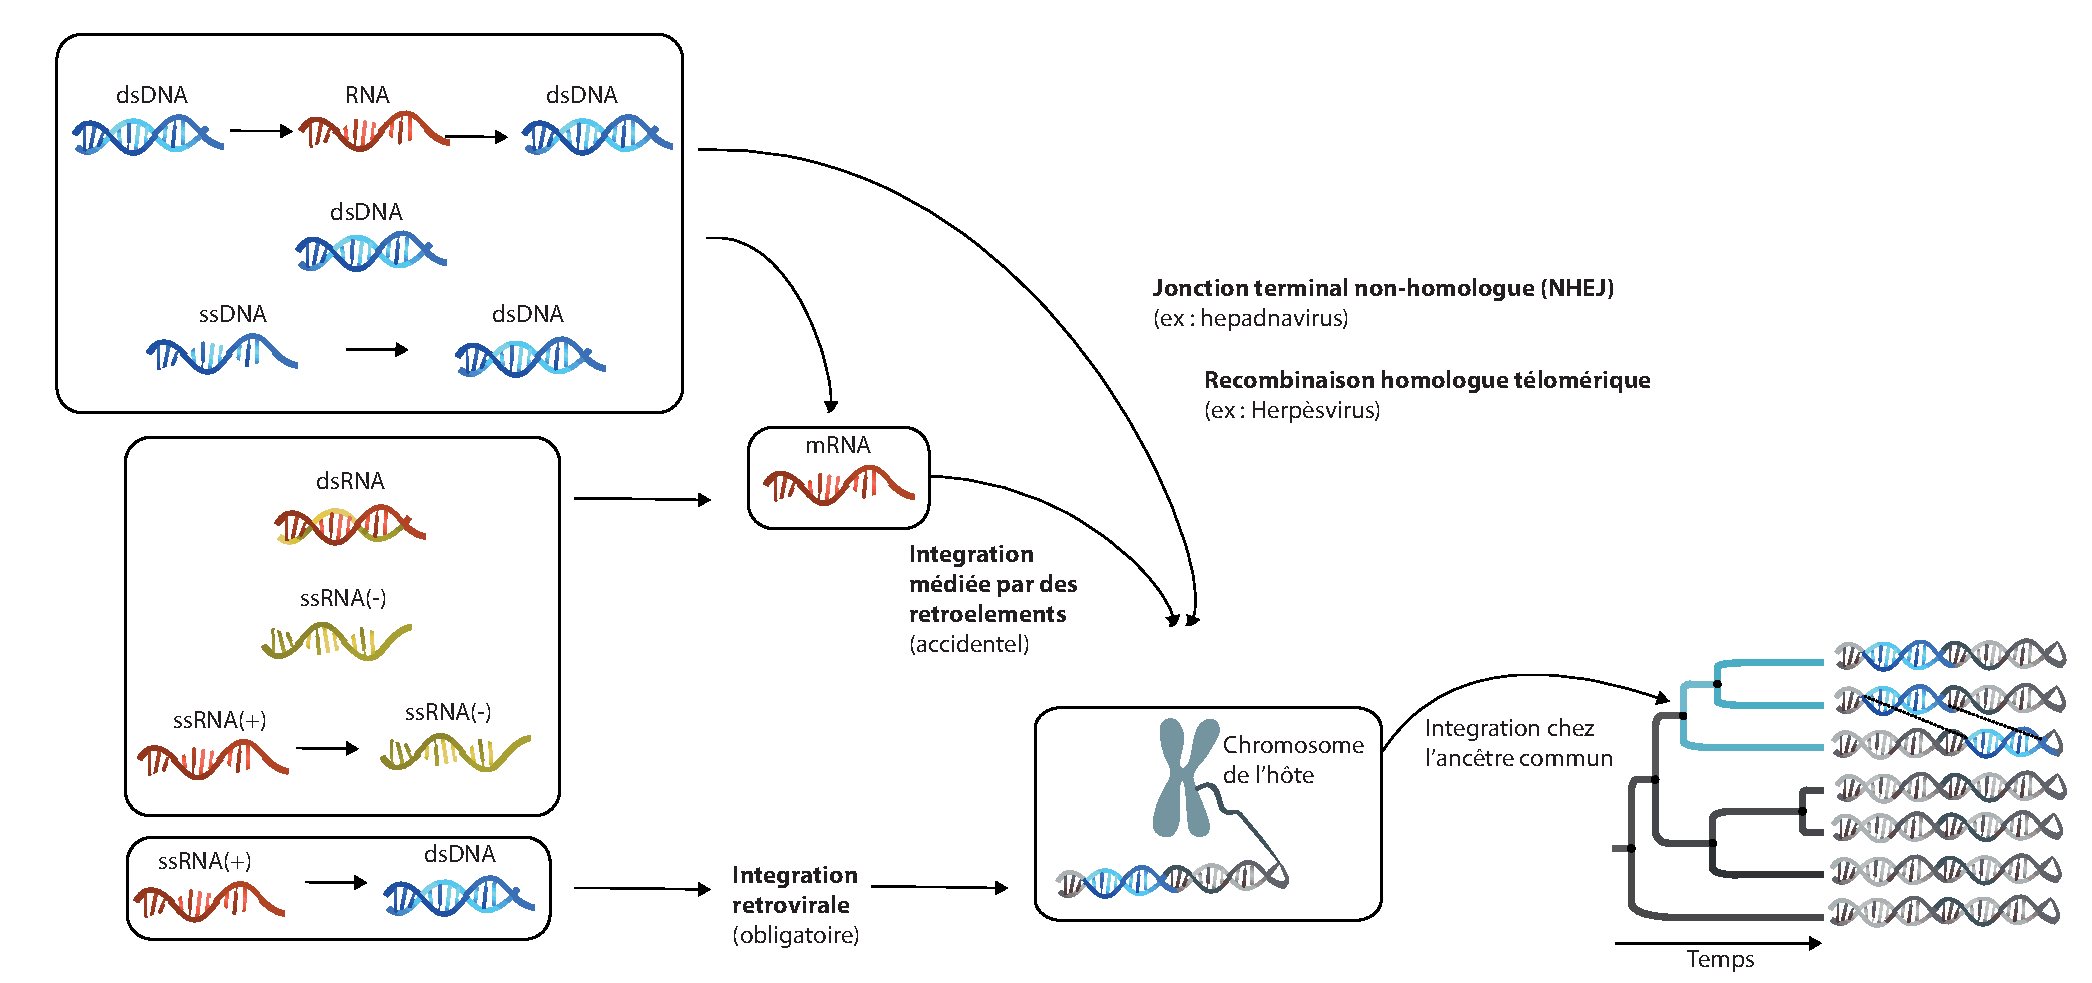
\includegraphics[width=\linewidth,height=\textheight,keepaspectratio]{PhD-master/figures/EVEs.pdf}
\caption[Intro:Schéma récapitulatif d'endogénisation virale]{\textbf{Schéma récapitulatif d'endogénisation virale modifié de \cite{katzourakis_endogenous_2010}}. Lorsqu'un évènement d'endogénisation viral a lieu dans le chromosome d'une cellule germinale d'une espèce, ces EVEs peuvent se voir transmis à la descendance et se fixer dans la population. L'histoire évolutive de ces EVEs doit alors être congruente avec l'histoire évolutive des hôtes. Plus l'évènement est ancien, plus nous pouvons nous attendre à observer des épisodes de réarrangement ou de pertes au cours de l'évolution.}
\label{figure:EVE}
\end{figure}



\subsection{Naissance d'un EVE}

L'apparition des EVEs peut donc survenir suite à l'intégration chromosomique de l'ADN viral (ou de copies d'ADN complémentaires issues d'ARN viraux) médiée par plusieurs mécanismes. Néanmoins, ces évènements sont rares chez les eucaryotes puisque d’une part l’ADN est protégé par un noyau, ce qui rend les contacts entre des éléments génétiques exogènes et le génome plus difficiles, et d’autre part, chez les espèces métazoaires tout au moins, la lignée germinale est habituellement séparée du reste des cellules, un gène acquis chez un métazoaire n’a donc aucune chance d'être fixé dans une population s’il n’atteint pas la lignée germinale. Aussi rares soient-ils, de tels évènements d'intégration germinale peuvent néanmoins survenir, monter en fréquence, puis se fixer dans la population  (\figurename{\ref{figure:EVE}}). Ces fixations peuvent se produire de manière non adaptative, par dérive, ou dans un certain nombre de cas, à la suite de processus adaptatifs. On parle alors de domestication virale que je vais illustrer dans la partie 2.3. 

\subsection{Les EVEs : des fossiles pouvant dater l'histoire ancienne des virus} 

Les séquences génomiques virales accumulent des changements évolutifs à un rythme élevé en raison de leur taux d'évolution élevé. Sur le temps ancien, du fait de la saturation du signal, les séquences virales contemporaines ne portent donc qu'une quantité limitée d'informations. En conséquence, les données virales contemporaines sont souvent insuffisantes pour nous informer sur la façon dont les virus ont évolué et ont interagi avec leurs hôtes dans les temps très anciens. Il n'existe par ailleurs pas de trace fossile de ces virus. Néanmoins, les virus peuvent laisser des empreintes durables dans les génomes de leurs hôtes à travers ces événements d'endogénisation. Après ces évènements, les génomes viraux ne sont plus soumis aux taux de mutation très élevés des virus (\figurename{\ref{figure:Taille_et_mutations_virales}} et \figurename{\ref{figure:Datation_virale_et_taux}}); au contraire, ils sont désormais liés aux génomes de leurs hôtes, dont les taux de mutation sont beaucoup plus faibles \citep{katzourakis_endogenous_2010, feschotte_endogenous_2012} (\figurename{\ref{figure:Datation_virale_et_taux}}). 

\begin{figure}[!htpb]
\captionsetup{font=footnotesize}
 \centering
  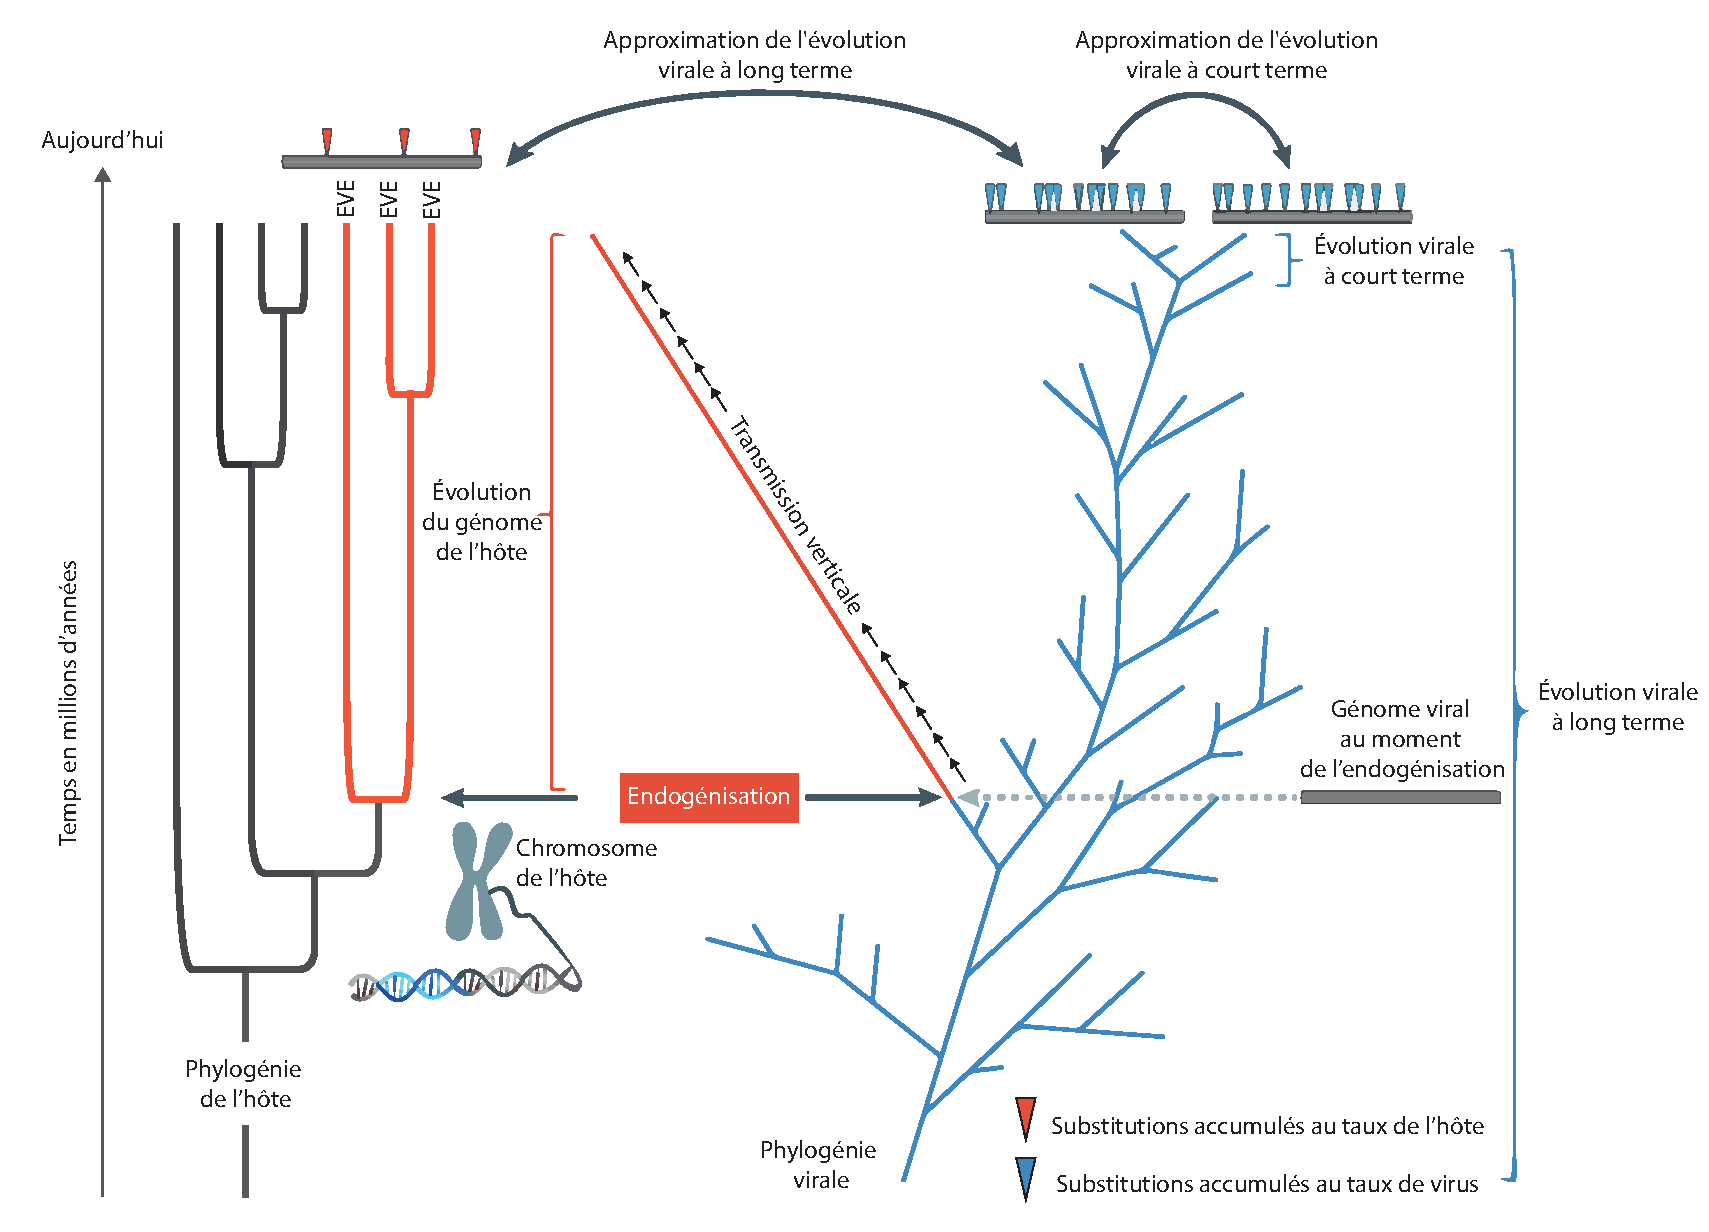
\includegraphics[width=\linewidth,height=\textheight,keepaspectratio]{PhD-master/figures/Datation_virale_et_taux.pdf}
\caption[Intro:Schéma du principe de datation des EVEs ]{\textbf{Datation des EVEs et déduction des taux de substitution virale à long terme modifié de \cite{feschotte_endogenous_2012}}. Lors d'un évènement d'endogénisation d'un virus chez l'ancêtre commun de plusieurs espèces eucaryotes, les séquences intégrées vont se mettre à évoluer au même rythme que les séquences du génome eucaryote (rouge). Tandis que les virus apparentés au donneur de ces EVEs vont eux continuer à évoluer avec de forts taux de mutations (bleu). Si nous voulons dater l'arbre viral, nous pouvons donc utiliser les informations de l'âge relatif des nœuds disponibles dans l'arbre eucaryote récoltés par exemple à partir de fossiles. Ces nœuds peuvent nous permettre de calibrer l'arbre viral puisqu'il existe toujours une relation phylogénétique entre les EVEs et les séquences virales contemporaines.}
\label{figure:Datation_virale_et_taux}
\end{figure}

Les EVEs fixés conservent donc des informations sur la circulation des virus anciens, qu'il est parfois impossible de déduire de l'examen des populations virales contemporaines. Ils fournissent des informations essentielles sur les virus anciens, telles que leur gamme d'hôtes, les échelles de temps d'évolution, ou les répartitions géographiques \citep{gifford_transitional_2008,katzourakis_endogenous_2010}.

Il existe ainsi diverses méthodes qui permettent d'utiliser les informations provenant des EVEs pour donner une limite inférieure sur l'âge des familles virales concernées \citep{aiewsakun_endogenous_2015}. L'une d'entre elle, applicable à tous les types de virus endogènes, consiste à exploiter les informations provenant d'EVEs orthologues (c'est-à-dire des EVEs hérités d'un ancêtre commun). Si la date de spéciation de ces espèces hôtes est par ailleurs connue grâce à des registres fossiles, il est alors possible de déduire que la date d'intégration du virus est antérieure à la spéciation des espèces hôtes concernées. 

Les lentivirus, par exemple, ont initialement été considérés comme un groupe de virus d'évolution récente, sur la base des origines très récentes du VIH-1 et des taux de substitution mesurés qui situent les origines des lentivirus à quelques milliers d'années \citep{sharp_origins_2000}. Pourtant, des chercheur.euse.s ont pu observer la présence de lentivirus endogénisés partagés dans des génomes apparentés de lapins, de furets, de lémuriens de Madagascar et de Colugos soutenant l'hypothèse d'une circulation de ces virus chez l'ancêtre de ces différents organismes, plusieurs millions d'années en arrière donc \citep{hron_life_2016,katzourakis_discovery_2007}. D'autres exemples analogues abondent comme chez les filovirus, parvovirus, circovirus, bornavirus, pestivirus, flavivirus qui circulaient déjà, il y a des millions d'années, au cours de l'évolution des mammifères, d'après leur distribution dans les espèces contemporaines \citep{katzourakis_endogenous_2010,taylor_filoviruses_2010,li_endogenous_2022}.

\begin{figure}[!htpb]
\captionsetup{font=footnotesize}
 \centering
  \includegraphics[width=\linewidth,height=\textheight,keepaspectratio]{PhD-master/figures/Datation_virale_scheme.pdf}
\caption[Intro:exemple de datation virale à partir d'EVEs]{\textbf{exemple d'une phylogénie virale calibrée à partir de virus domestiqués modifié de \cite{theze_paleozoic_2011}}. Dans cet exemple, la phylogénie des virus à grand génome à ADN double brin infectant les arthropodes de la classe des \textit{Naldaviricetes} a pu être calibrée grâce à un évènement d'endogénisation ayant eu lieu y a environ 100 millions d'années chez l'ancêtre commun des guêpes parasitoïdes appartenant au complexe des Microgastroïdes.}
\label{figure:Datation_virale_scheme}
\end{figure}

Dans un autre exemple, \cite{theze_paleozoic_2011} ont  pu exploiter les EVEs partagés par plusieurs milliers d'espèces d'Hymenoptères parasitoïdes (le complexe microgastroïde au sein des Braconidae) pour calibrer la phylogénie des virus donneurs (\figurename{\ref{figure:Datation_virale_scheme}}). Cette calibration permet en retour de dater la divergence de la famille de virus. En effet, grâce à l'étude de \citep{murphy_phylogeny_2008}, les chercheur.euses savaient que le temps jusqu'à l'ancêtre commun le plus récent de l'espèce \textit{Chelonus inanitus} et de \textit{Cotesia congregata} était égal à 103,38 +/- 4,41 Mya (correspondant au nœud 2 dans la \figurename{\ref{figure:Datation_virale_scheme}}). De même, ils savaient que l'ancêtre commun de \textit{Cotesia congregata} et de \textit{Toxoneuron nigriceps} était estimé à environ 87 +/- 5 Mya (nœud 1 dans la \figurename{\ref{figure:Datation_virale_scheme}}). Aussi, sur la base de ces estimations provenant de registres fossiles, ces points de calibration dans l'arbre de l'hôte (point 1 et 2) peuvent également servir de point de calibration dans l'arbre des virus (point 1 et 2) (\figurename{\ref{figure:Datation_virale_scheme}}). Une fois l'arbre viral calibré, la divergence entre la famille des \textit{Baculoviridae} et celle des \textit{Nudiviridae} a pu être estimée. Ces analyses révèlent que les virus dsDNA des insectes (ici représentés par les \textit{Nudiviridae} et \textit{Baculoviridae}) se seraient diversifiés il y a environ 310 Mya à l'ère paléozoïque, pendant la période carbonifère, ce qui coïncide avec la période de diversification des premiers ordres d'insectes \citep{theze_paleozoic_2011}. 

\section{Les Éléments viraux endogènes domestiqués (dEVEs)}

Quel est le devenir des éléments endogénisés ? La dégénérescence est probablement le destin le plus fréquent des EVEs, puisqu'il s'agit d'un évènement de mutation accidentel qui n'apporte \textit{a priori} aucun bénéfice pour l'hôte. En effet, de nombreux EVEs identifiés ont accumulé un grand nombre de mutations depuis leur intégration et/ou sont fragmentés : ils représentent probablement des pseudogènes non fonctionnels, évoluant sous un régime neutre \citep{katzourakis_endogenous_2010}. Cependant, l'endogénisation de séquences virales dans le génome de l'hôte peut parfois être bénéfique pour l'hôte et entraîner une fixation de l'élément viral endogène dans les populations à travers un phénomène de sélection positive.  On parle alors de domestication et les EVES sont qualifiés de dEVEs (pour domesticated Endogenous Viral Elements) \citep{koonin_depths_2018}. Ainsi, l'introduction d'un ou plusieurs gènes viraux dans les génomes eucaryotes représente un input mutationnel à fort impact. En effet, ces mutations peuvent être vues comme des "macro-mutations" dans la mesure où un ou plusieurs gènes déjà fonctionnels et façonnés par la sélection naturelle sont intégrés, ce qui offre de nombreuses possibilités de domestication par l'hôte. Les travaux sur la domestication des EVEs ont permis d'identifier de nombreuses fonctions recrutées par les eucaryotes, telles que des fonctions de communication et d'échanges métaboliques, de défenses antivirales, de plasticité phénotypique ou bien les interactions hôtes-parasites. 

\subsection{Développement placentaire}

Les exemples les mieux étudiés jusqu'à présent sont les protéines syncytines. Ces protéines retrouvées chez tous les mammifères placentaires sont dérivées de protéines \textit{env} présentes chez des rétrovirus. Les rétrovirus ciblent, se fixent et intègrent les membranes des cellules cibles en exprimant le gène \textit{env} (Coffin JM et al., 1997). Ces protéines ont des propriétés fusogéniques et permettent aux virus de se lier aux celles de leurs hôtes. De manière remarquable, cette protéine a été domestiquée à plusieurs reprises chez plusieurs lignées de mammifères et de lézards vivipares et permet la formation du syncitium en médian une fusion entre les cellules de la mère et de l'embryon permettant les échanges métaboliques entre la mère et le fœtus (\figurename{\ref{figure:Syncitine_illustration}}-A) \citep{lavialle_paleovirology_2013,cornelis_endogenous_2017}. En effet, ces gènes sont domestiqués dans toute la sous-classe des thériens, avec au moins dix événements d'intégration rétrovirale indépendants \citep{imakawa_baton_2015}(\figurename{\ref{figure:Syncitine_illustration}}-B).\\

De manière surprenante, les propriétés fusogéniques des syncytines semblent également avoir été  utilisées pour soutenir le développement musculaire, car le knock-out de la syncytine B chez les souris entraîne une diminution de la fusion des myoblastes et de la masse musculaire chez les mâles \citep{redelsperger_genetic_2016}. Ces résultats montrent comment les propriétés biochimiques des enveloppes virales ont été recyclées plusieurs fois au cours de l'évolution.

\begin{figure}[H]
\captionsetup{font=footnotesize}
 \centering
  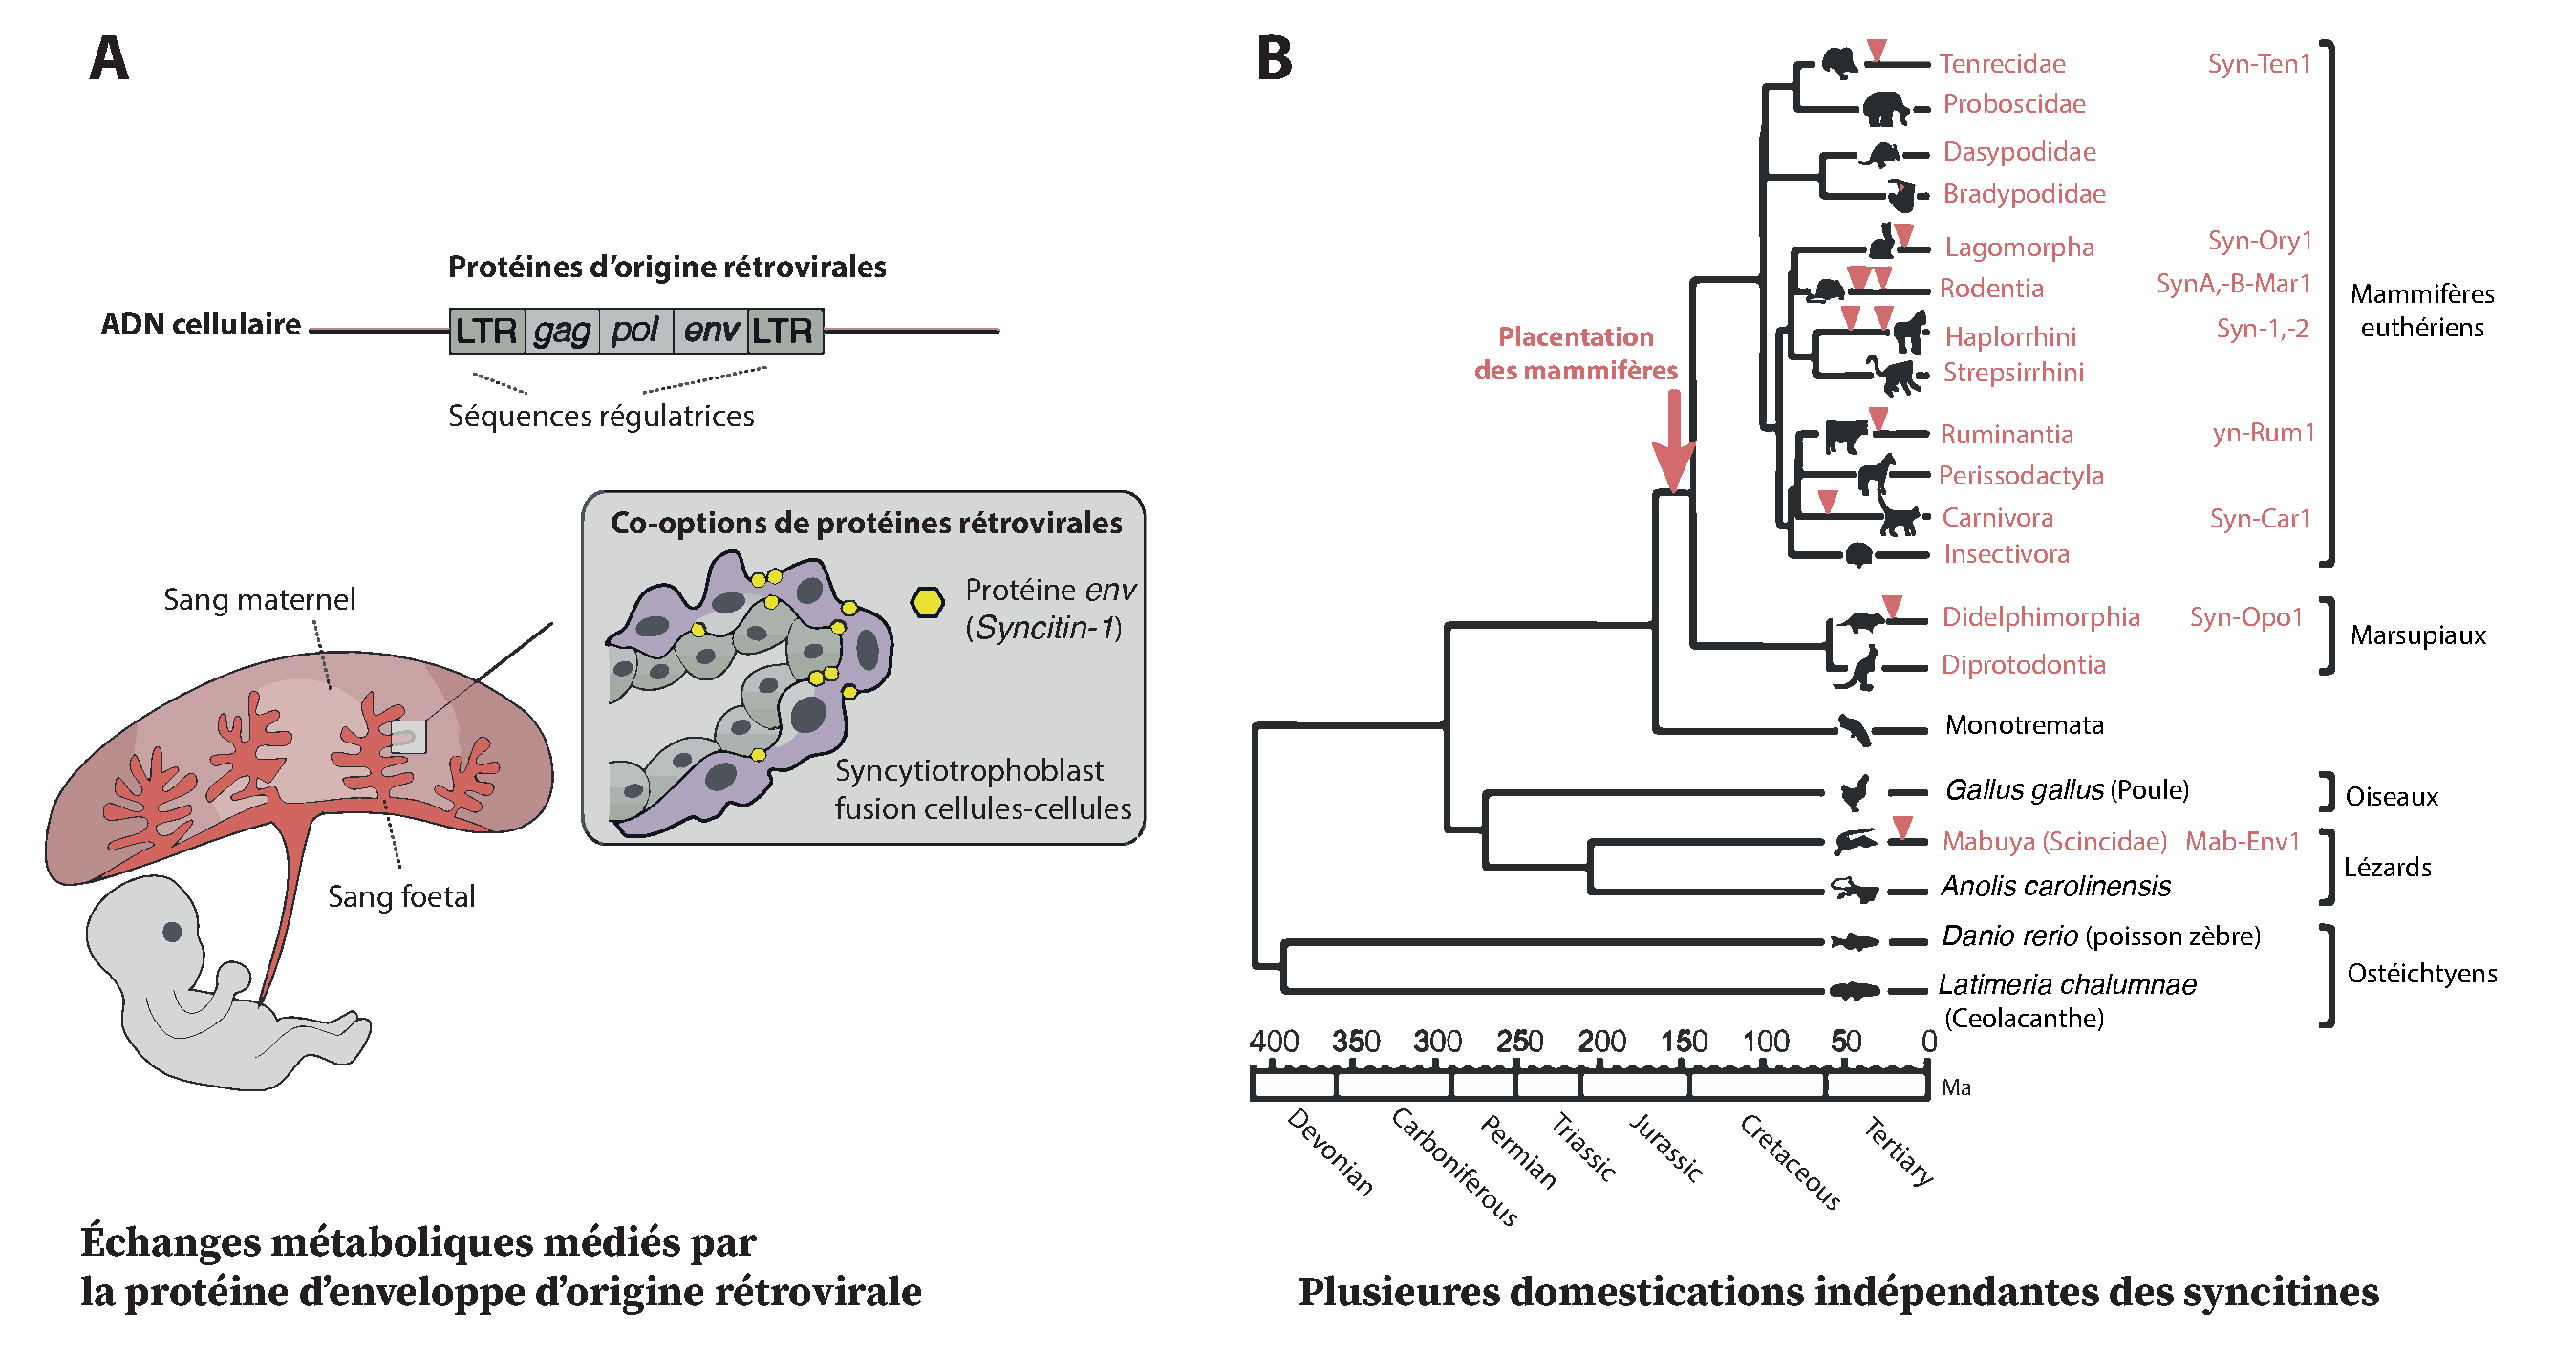
\includegraphics[width=\linewidth,height=\textheight,keepaspectratio]{PhD-master/figures/Syncitine_illustration.pdf}
\caption[Intro:Illustration d'un gène de rétrovirus impliqué dans la production du syncitium chez les mammifères placentaires]{\textbf{Exemple schématique de la domestication d'un gène rétroviral impliqué dans la formation du syncytium modifié de} \cite{chuong_placenta_2018, cornelis_endogenous_2017}. \textbf{A} -  Exemple schématique de la fonction fusogénique des syncitines dans la formation du syncytiophoblast ainsi que la disposition des gènes rétroviraux et de séquences régulatrices le long du génome d'un mammifère. \textbf{B} -  Classification des mammifères, du lézard \textit{Mabuya} et des syncytines connues selon la phylogénie des vertébrés. Les mammifères comprennent les monotrèmes (p. ex. l'ornithorynque) qui produisent encore des œufs, ainsi que les marsupiaux et les mammifères euthériens qui ont un placenta (caractères rouges). Le lézard \textit{Mabuya} est représenté en rouge, car il porte lui aussi un placenta. Une flèche rouge marque la période probable de formation du placenta des mammifères, qui a été supposée correspondre à la capture d'une syncytine ancestrale, qui a ensuite été remplacée par les syncytines actuelles présentées. Toutes les occurrences de capture de syncytine actuellement décrites sont indiquées par des pointes de flèche rouges à côté du nom de la syncytine. Comme l'illustre l'échelle située sous l'arbre, la longueur des branches est liée au temps en millions d'années.}
\label{figure:Syncitine_illustration}
\end{figure}

\subsection{La communication synaptique}

Un autre fait remarquable de domestication virale impliquant des rétrovirus est celui du gène neuronal \textit{Arc}. Ce gène est dérivé d'un rétrotransposon Ty3/Gypsy domestiqué et code un domaine de capside présentant une similarité structurelle avec les protéines rétrovirales. Récemment, il a été  démontré que cette protéine forme des structures de type capside, impliquées dans la fonction neuronale et la mémoire \citep{ashley_retrovirus-like_2018}, Ces protéines, à la façon d'un rétrovirus (\figurename{\ref{figure:Arc_illustration}}-A), s'auto-assemble en capsides de type viral capables d'encapsider de l'ARN (\figurename{\ref{figure:Arc_illustration}}-B). Ces capsides permettent de réguler la plasticité synaptique en médian des échanges synaptiques. Ensuite, la protéine Arc endogène est libérée des neurones dans des vésicules extracellulaires, facilitant le transfert de l'ARNm \textit{Arc} dans de nouvelles cellules musculaires post-synaptiques  où il est traduit en protéine \citep{ashley_retrovirus-like_2018, pastuzyn_neuronal_2018}. 
Tout comme la syncytine chez les mammifères, les gènes \textit{Arc} retrouvés chez les drosophiles et les tétrapodes descendraient de plusieurs évènements d'endogénisation indépendants de rétrotransposons Ty3/gypsy dans des lignées eucaryotes distinctes \citep{pastuzyn_neuronal_2018}. \\

\begin{figure}[H]
\captionsetup{font=footnotesize}
 \centering
  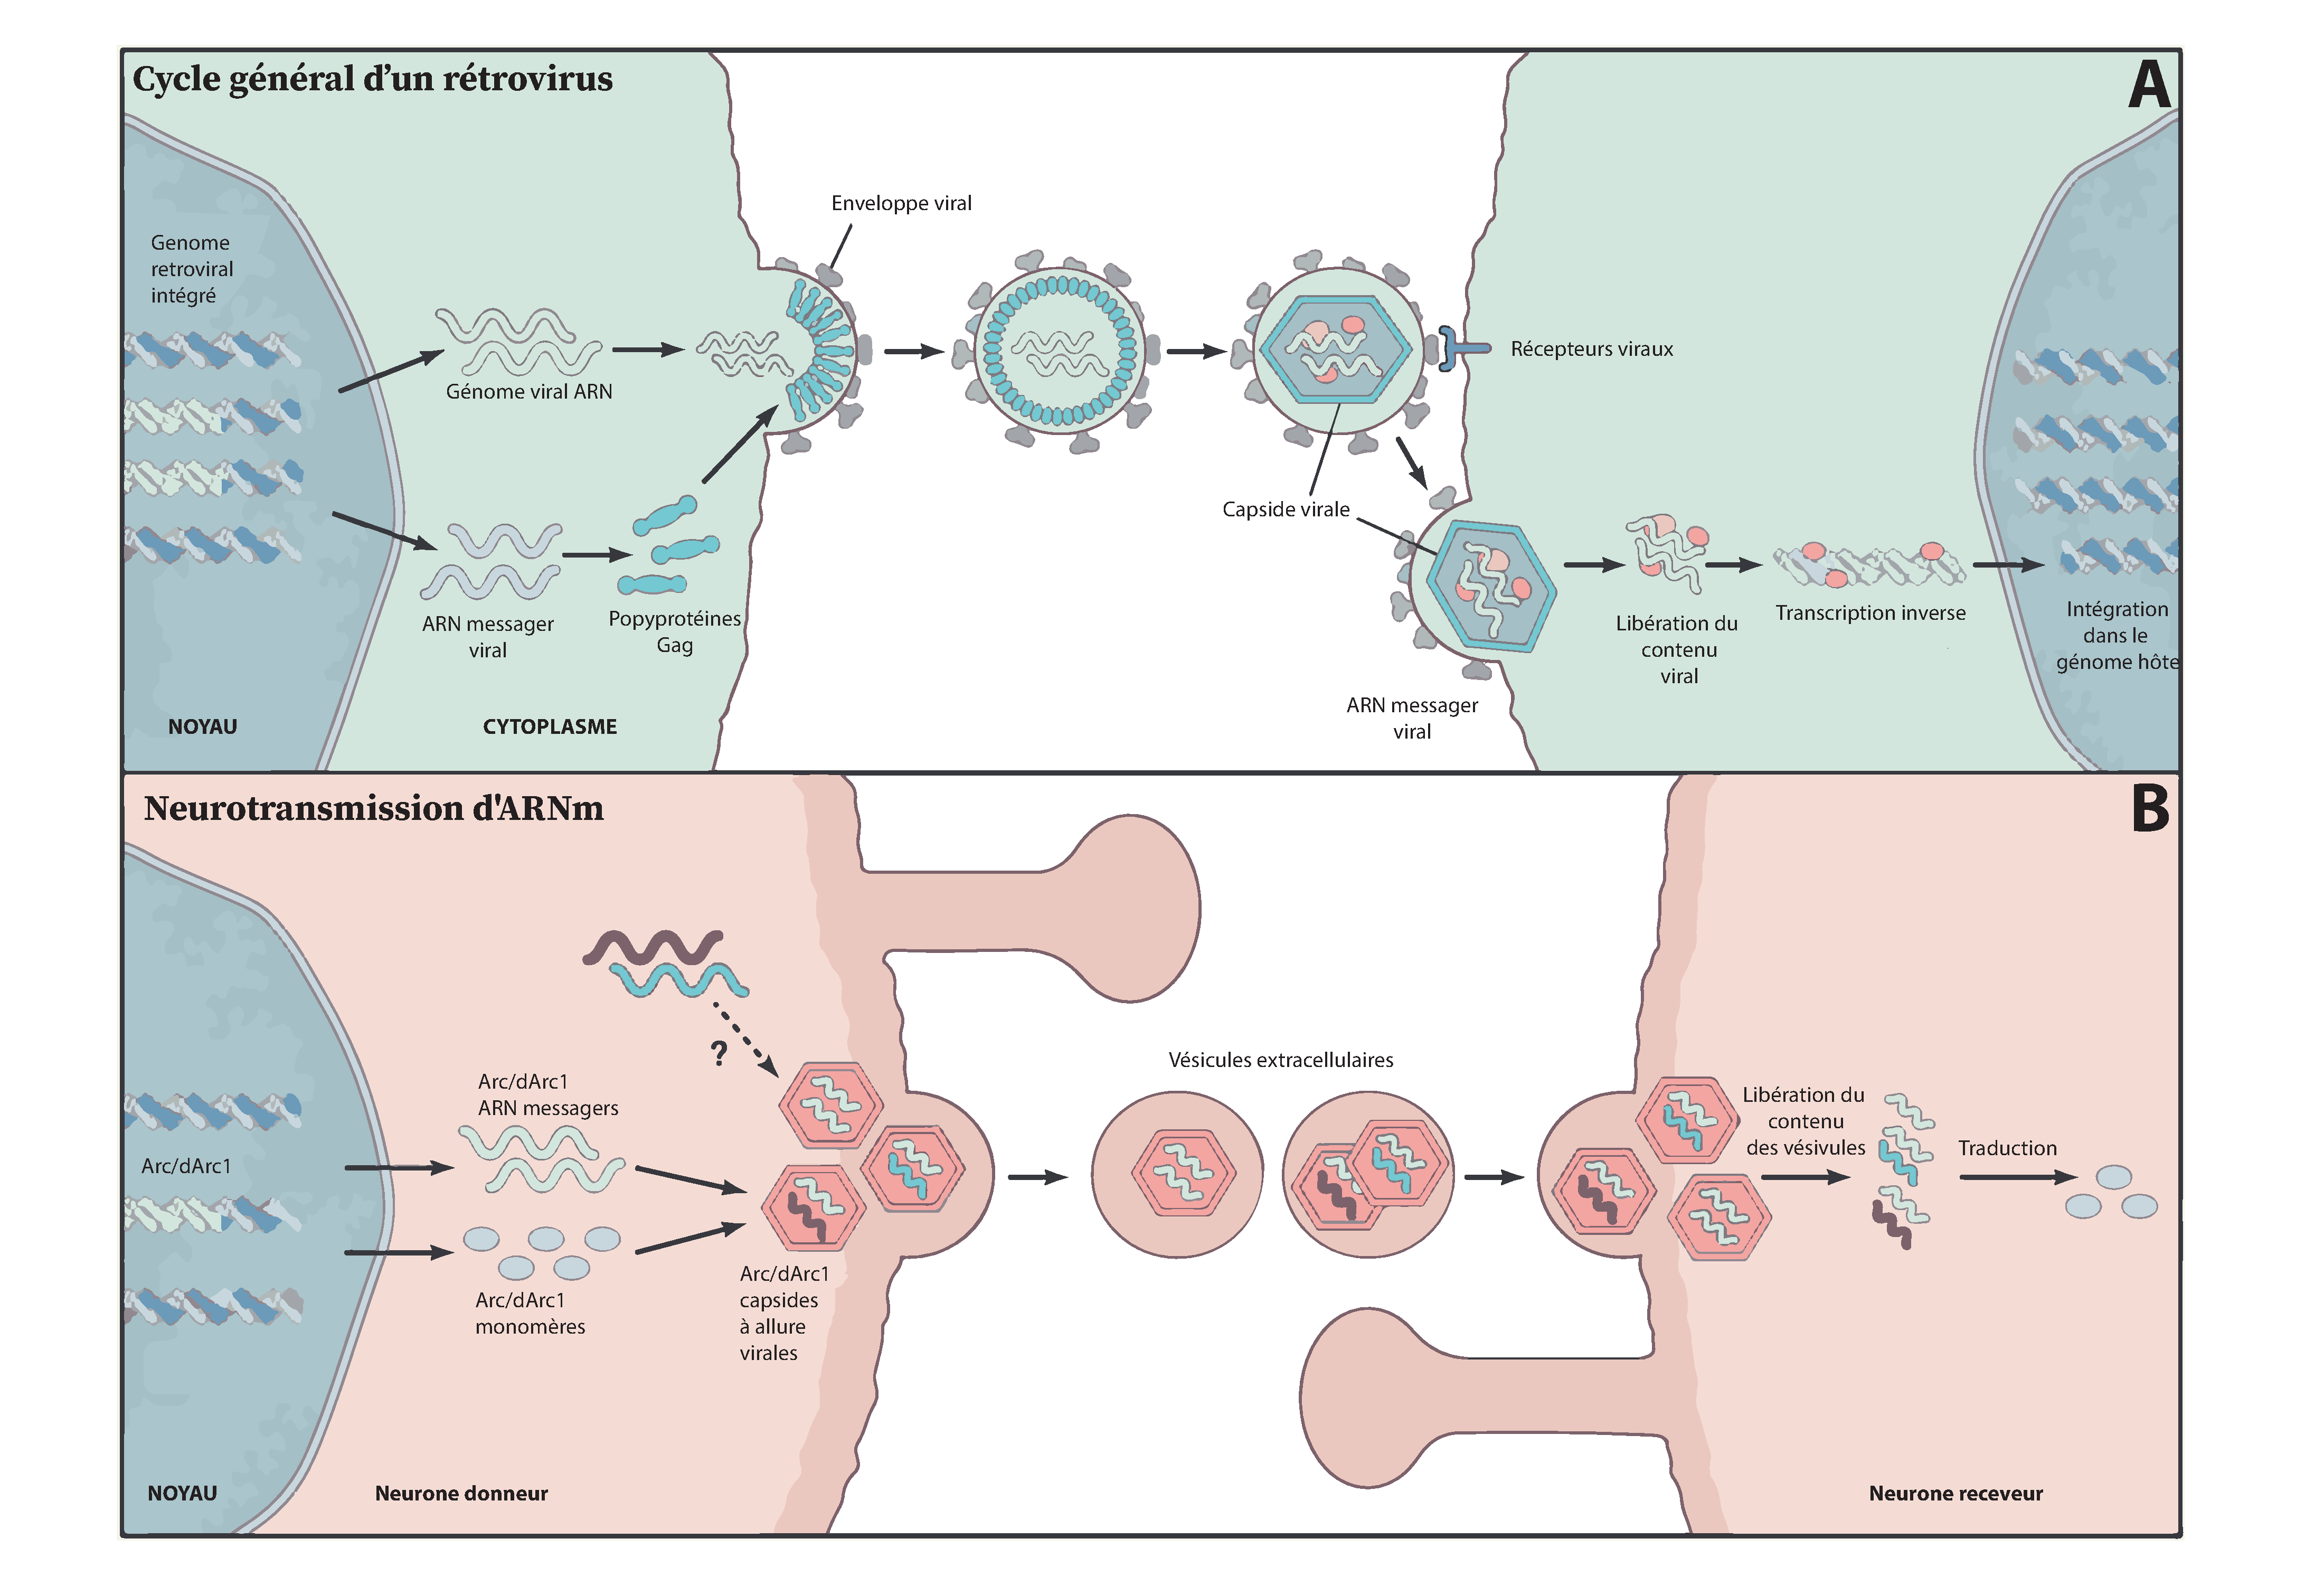
\includegraphics[width=\linewidth,height=\textheight,keepaspectratio]{PhD-master/figures/Arc_illustration.pdf}
\caption[Intro:Illustration de la fonction du gène rétroviral \textit{Arc}]{\textbf{Illustration de la fonction du gène rétroviral \textit{Arc} modifié de \cite{parrish_viral_2018}}. \textbf{A} - Cycle rétroviral classique dans lequel la polyprotéine rétrovirale \textit{Gag} assure la formation de la capside afin de regrouper les génomes viraux et de les transférer dans le cytoplasme des cellules nouvellement infectées. \textbf{B} - L'oligomérisation des protéines \textit{Arc} de souris et \textit{Arc1} de drosophile (\textit{dArc1}) forme des capsides ressemblant à celles des virus. Les capsides \textit{Arc/dArc1} sont libérées des neurones dans des vésicules extracellulaires, où elles transmettent leurs ARNm associés (vert clair) et peut-être des ARN supplémentaires (marron, bleu) à la synapse ou à la jonction neuromusculaire.} 
\label{figure:Arc_illustration}
\end{figure} \newpage

\subsection{Immunité antivirale}

 Le principal mécanisme antiviral chez les arthropodes est l'interférence ARN (ARNi), qui repose sur trois types de petits ARN (ARNs : siARN, miARN et piRNA) \citep{obbard_evolution_2009}. La voie du petit ARN interférent (siARN) est la branche la plus importante de l'ARNi pour combattre l'infection virale chez les arthropodes. Elle repose sur le clivage du génome viral pour produire principalement des siRNA de 21 nucléotides \citep{obbard_evolution_2009}. Ces siRNA se lient aux protéines Argonaute, ce qui dirige le complexe multiprotéique de silencing vers l'ARN viral, entraînant ainsi le clivage endonucléolytique de l'ARN viral cible. La voie des microARN (miRNA) repose principalement sur l'appariement imparfait des bases entre les miRNA et les ARN viraux pour inhiber la traduction. Toutefois, les miRNA peuvent aussi diriger le clivage de l'ARN cible s'il existe une complémentarité suffisante entre le miRNA et l'ARN cible \citep{obbard_evolution_2009}. Un troisième type d'ARNi, dirigé par des ARN interagissant avec le complexe PIWI (piRNA), a récemment été découvert. La fonction principale de la voie des piRNA est de contrôler les éléments transposables dans les cellules germinales animales pour prévenir les effets délétères des événements de transposition \citep{cosby_hosttransposon_2019}. Seulement, la production \textit{de novo} de piRNA dérivés de séquences virales endogénisées a également été observée chez les moustiques \textit{Aedes aegypti} et \textit{Ae. albopictus}. La production de ces piRNA dérivant de virus pourrait donc également servir de médiateurs à l'immunité antivirale en ciblant des ARN viraux exogènes présentant des niveaux élevés d'identité de séquence\citep{miesen_piwis_2016} (\figurename{\ref{figure:Antiviral_immunity}}).\\

Bien que les EVEs aient été observés dans une variété d'autres espèces d'arthropodes, leur implication possible dans la voie piRNA reste inconnue et semble limitée aux moustiques du genre \textit{Aedes} \citep{ter_horst_endogenous_2019, cerqueira_de_araujo_transposable_2022}.\newpage

\begin{figure}[!htpbt]
\captionsetup{font=footnotesize}
 \centering
  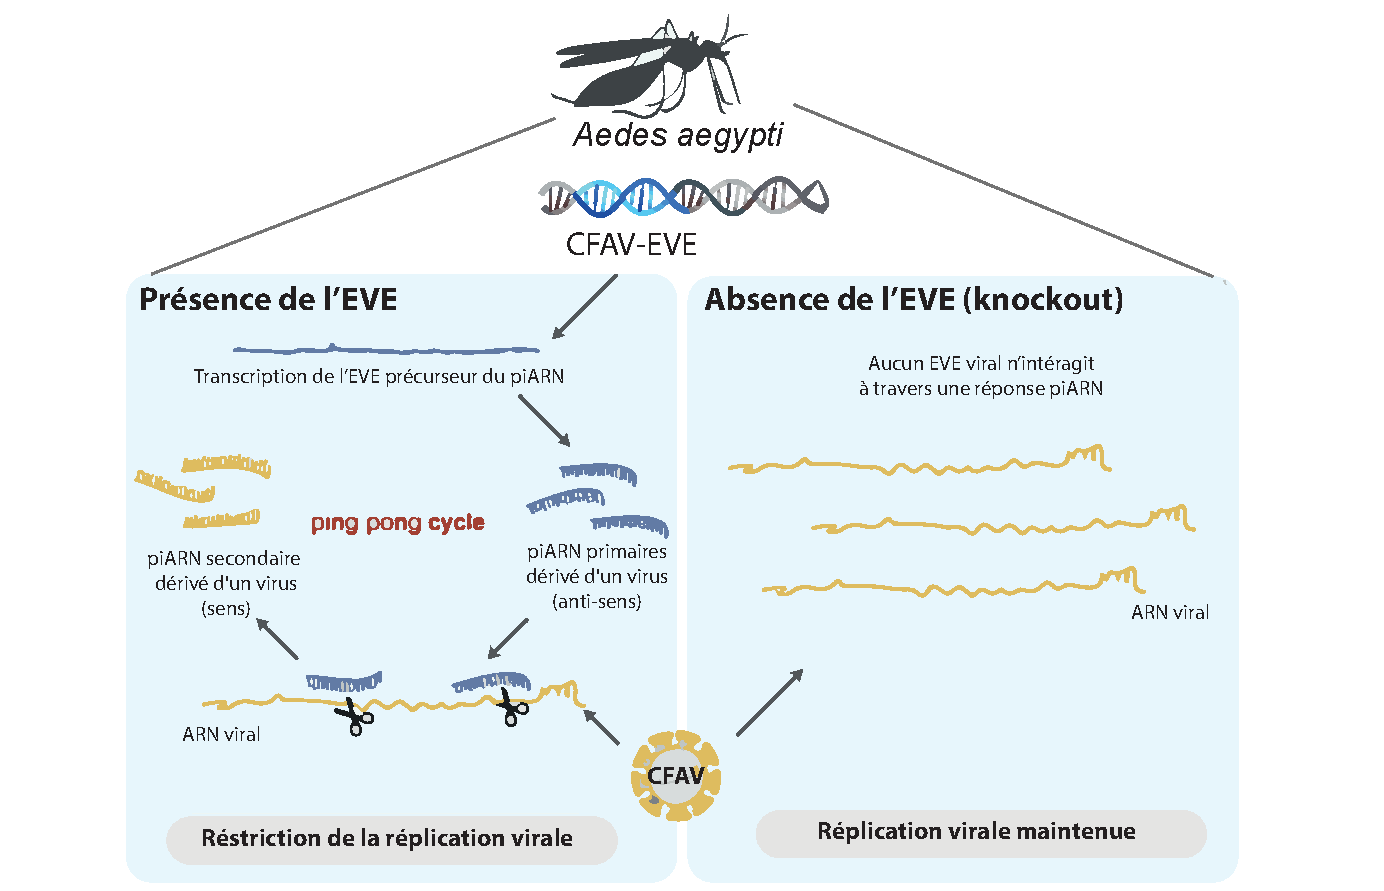
\includegraphics[width=\linewidth,height=\textheight,keepaspectratio]{PhD-master/figures/Antiviral_immunity.pdf}
\caption[Intro:Illustration d'un gène d'arbovirus impliqué dans l'immunité antivirale chez le moustique]{\textbf{Illustration d'un gène d'arbovirus impliqué dans l'immunité antivirale modifié de \cite{suzuki_non-retroviral_2020}}. La recherche systématique d'EVEs dans le génome des moustiques du genre \textit{Aedes} a révélé la présence de nombreuses EVEs au cœur même des clusters de piRNA (régions concentrées du génome produisant les piRNA).Ces clusters sont transcrits à partir des deux brins, et contiennent des centaines à des milliers de gènes de piRNA qui sont souvent organisés en réseaux en tandem. Ainsi, la présence d'EVEs en abondance dans ces régions  soulève la possibilité  que les EVEs participent à une réponse antivirale contre les virus exogènes via la voie des piRNA \citep{palatini_comparative_2017,suzuki_uncovering_2017}. Dans cette fameuse voie, une amplification réciproque des piRNA est effectuée lors d'un cycle ping-pong. Dans ce cycle, les transcrits anti-sens de piRNA précurseur sont produits à partir d'une matrice provenant de l'EVE. Ces transcrits guident le clivage des séquences d'ARN complémentaires qui proviennent d'un virus infectieux suffisamment proche en termes de séquence. S'ensuit le recrutement de complexes protéiques permettant de couper le transcrit viral en plusieurs morceaux. Ces transcrits de piRNA secondaires dérivés du virus induisent ensuite le clivage des transcrits précurseurs de piRNA, transformés ensuite en piRNA primaire, et ainsi de suite, ce qui empêche le virus infectieux de se répliquer correctement.}
\label{figure:Antiviral_immunity}
\end{figure}

\subsection{Réponse à un changement de condition environnementale}

En réponse à des changements environnementaux, certains organismes peuvent modifier leur phénotype, on appelle cela de la plasticité phénotypique. Ce phénomène peut se produire à différents niveaux, du niveau cellulaire au niveau de l'organisme, et même au niveau de la population.

Les pucerons constituent un exemple classique de plasticité phénotypique face à des variations de densité. En cas de surpopulation, certains individus produisent des progénitures ailées. Les pucerons ailés peuvent se disperser dans de nouveaux environnements, mais cela a un coût : ils produisent moins de descendants que leurs homologues dépourvus d'ailes \citep{sutherland_role_1969}. Ainsi, la valeur adaptative d'un individu est déterminée par sa capacité à détecter les conditions environnementales et à y répondre efficacement. 

Chez les clones asexués du puceron rose du pommier (\textit{Dysaphis plantaginea}), la production de la forme ailée est fortement accentuée par l'infection par un densovirus : Dysaphis plantaginea densovirus (DplDNV) \citep{ryabov_densovirus_2009}. En réponse à la surpopulation, dans les conditions expérimentales de l'étude, seuls les clones infectés par le virus ont produit des progénitures ailées, bien qu'ils en aient produit moins que les clones non-infectés \citep{ryabov_densovirus_2009}(\figurename{\ref{figure:Pucerons_densovirus}}-B). 

Ainsi, dans ce système, les virus contribuent à leur propre  dispersion en maximisant la dispersion de leurs hôtes à travers la formation d'individus ailés, mais contribuent peut-être également à la fitness des pucerons en leur permettant de se reproduire sur de nouveaux patchs de ressources. 

De manière remarquable, le puceron du pois (\textit{Acyrthosiphon pisum}, une espèce cousine de \textit{D.plantaginea}) (\figurename{\ref{figure:Pucerons_densovirus}}-A), présente les mêmes phénotypes de dispersion, mais chez ce dernier, c'est la domestication directe de deux gènes de densovirus qui est impliquée dans la plasticité de ce phénotype ailé\citep{parker_laterally_2019} (\figurename{\ref{figure:Pucerons_densovirus}}-C). En effet, à l'intérieur du génome de \textit{A.pisum}, deux gènes fortement exprimés en condition de promiscuité forte, (\textit{Apns-1} et \textit{Apns-2}), ont été découverts. Ces gènes sont en réalité des EVEs dérivant de gènes non structuraux d'un densovirus apparenté à (DplDNV) \citep{parker_laterally_2019}. Ainsi, les génotypes fortement inductibles expriment les gènes \textit{Apns} plus fortement que les génotypes faiblement inductibles, favorisant ainsi la dispersion des pucerons et permettant d'échapper aux conditions de promiscuité (\figurename{\ref{figure:Pucerons_densovirus}}-C).


\begin{figure}[!htpbt]
\captionsetup{font=footnotesize}
 \centering
  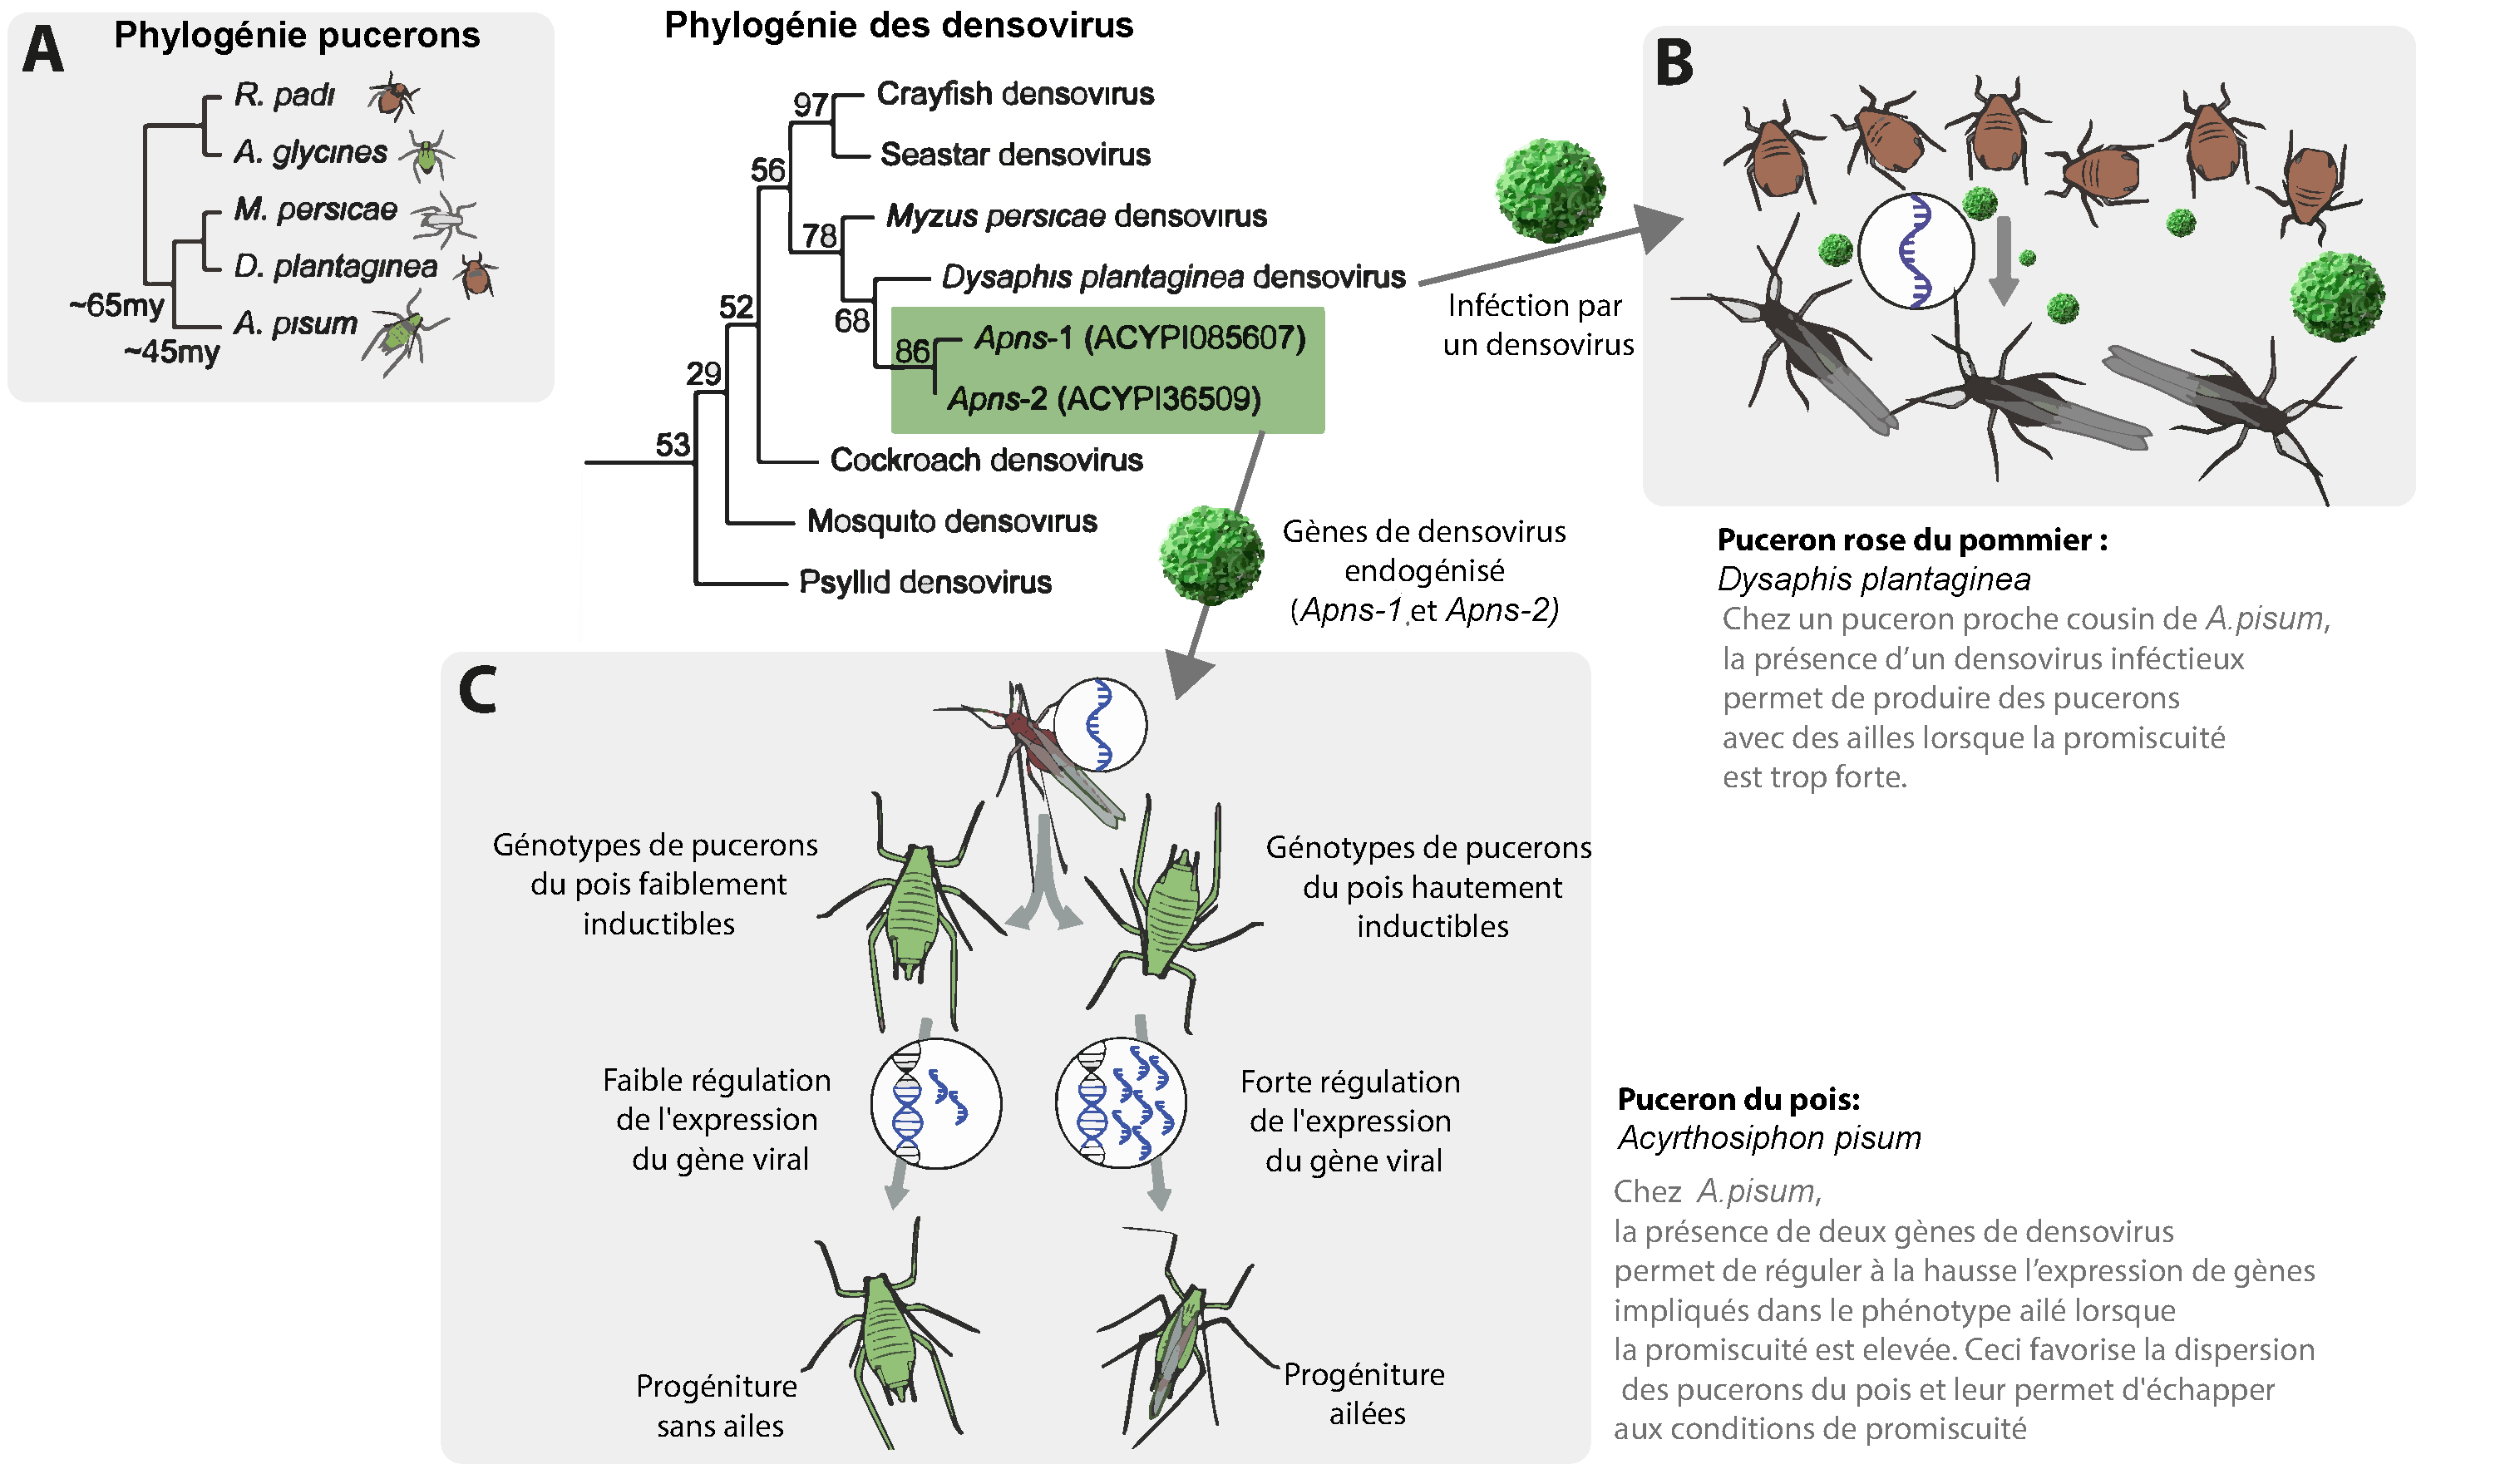
\includegraphics[width=\linewidth,height=\textheight,keepaspectratio]{PhD-master/figures/Pucerons_densovirus.pdf}
\caption[Intro:Illustration d'un gène de densovirus impliqué dans la plasticité phénotypique chez le puceron]{\textbf{Illustration d'un gène de densovirus impliqué dans la plasticité phénotypique modifié de \cite{parker_laterally_2019}}.}
\label{figure:Pucerons_densovirus}
\end{figure}


\subsection{Conclusion sur ces exemples de domestication}

Les évènements de domestication évoqués dans cette partie impliquent en général un nombre restreint de gènes viraux, souvent un seul. Dans la suite, nous allons nous intéresser à d'autres systèmes retrouvés chez des guêpes parasitoïdes. Ces systèmes impliquent la domestication d'une machinerie virale complexe agissant de concert pour produire et assembler des structures virales essentielles au succès reproducteur de ces guêpes. Les particules ainsi produites se nomment des polydnavirus (PDVs) et Virus-like particules (VLPs). À ma connaissance, parmi les organismes eucaryotes, seuls les PDVs et les VLPs domestiqués chez les guêpes parasitoïdes fournissent des exemples de domestication impliquant toute une machinerie virale.
